% 23 May 2001
%  	with corrections from Chris
% 30 May 2001 with corrections from Fred
% 30 May 2001 comments from Paola
% 30 May 2001 comments from R. Gomez
% 30 May 2001 comments from Steve

\chapter{Josephson-junction arrays as models of multiply-connected 
superconductors}
\label{chap:jjarray}

\section{Introduction}
\label{sec:jjarray_intro}

A typical sample of superconductor takes one of two general forms,
a single crystal, or a
polycrystal. Single crystals 
do not have grain boundaries
and by studying them we may learn many of the intrinsic superconducting 
properties.
However, only small single crystals can be grown.
This poses a problem industrially and experimentally. 
In industry, material must be manufactured in quantity
(\eg\ for wires) and fabricated
into devices (\eg\ \jjsnoun)
which cannot easily be done with a single crystal. Experimentally,
samples often need to be fabricated in a particular fashion
which may be
very difficult or impossible to do with a
single crystal.

Photo\-litho\-graphic
techniques make thin film samples ideal candidates for study because
samples may be fabricated of arbitrary geometry.
The use
of thin films adds several wrinkles to the study of superconductors. 
Thin films are polycrystalline and typically composed of randomly oriented
grains. 
In \hightc\ superconductors these grains can be quite disruptive, 
acting as \jjsnoun\ while in \lowtc\ the grain boundaries may not 
matter at all to the current flow. 
The grain boundaries behave as \jjsnoun --  two islands of 
superconductor joined by a weak link. Depending upon deposition 
conditions, superconducting grains may be randomly oriented and it may be
difficult to disentangle which sample properties result from granularity
and which result from island properties. 

Josephson-junction arrays are the 
quintessential multiply-connected superconductor. They 
can be photo\-lith\-o\-graph\-i\-cally realized and the equations 
that govern
Josephson-junction arrays are simple and well known.%
\footnote{See the review article by Newrock \etal\cite{newrock_ssp_54_263_2000}
for a more complete discussion of \jjsnoun\ and \jjas.}
Because of the control that photolithography gives
over sample fabrication,
Josephson-junction array samples may provide
important insight into the properties of granular superconductors.
By proper choice of \jja\ design one may create samples
to study the interrelationship between geometry and material
parameters of multiply-connected superconductors.

%
% fig 1
% 
\begin{figure}[p]
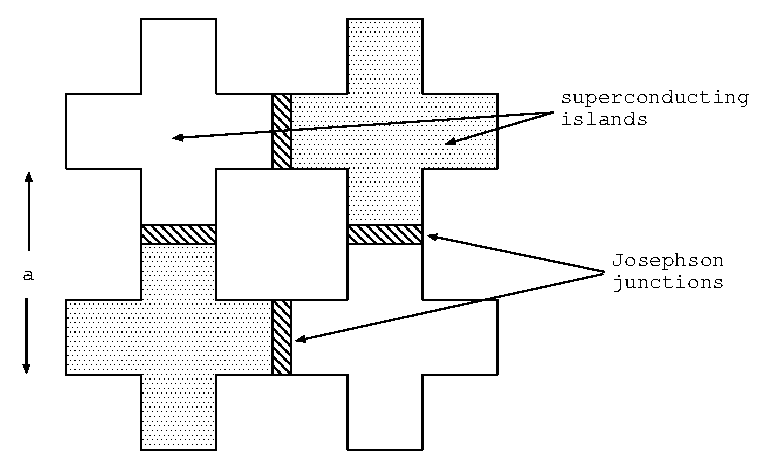
\includegraphics{figs/jjarray/fig1.eps}
\caption[One plaquette of a \jja.]{One plaquette of a \jja. The 
cross shaped islands of superconductor are in two layers 
(white and speckled). At the cross overlap a junction is formed
(cross-hatched region). The unit cell size is $a$. }
\label{fig:array_realization}
\end{figure}

\section{Single plaquette of Josephson-junction array}
\label{sec:single_loop}

Before analyzing the entire array in detail, I consider
the constitutive elements of the array: superconducting islands
joined by weak links, shown in \FigRef{fig:array_realization}.
The simplest component of the array is a single plaquette, a loop,
which 
for our arrays consists of four \jjsnoun, but in general may consist of
$N$ \jjsnoun. 
By looking at a single loop we can begin to 
directly compare experiment and 
analytical results. By contrast a
n entire array may only be solved numerically, 
even though the equations are known. 
Additionally, remnants of the single loop behavior may be seen
at the level of the entire array
\cite{ebner_prb_31_165_1985,deleo_unpublished}, 
so an understanding of the single-loop 
will be important to aid in understanding the entire array. 
Indeed the single-loop model has been used
many times in the literature in an attempt to explain phenomena
primarily associated with the paramagnetic Meissner effect
\cite{auletta_physc_235_3315_1994,araujo_prl_78_4625_1997,%
barbara_prb_60_7489_1999,sigrist_jpsj_61_4283_1992,sigrist_rmp_503_67_1995}. 

%
% fig2.2-- schemtic of RCSJ model
%
\begin{figure}[p]
\includegraphics{figs/jjarray/fig2.eps}
\caption[Circuit schematic of single \jjnoun.]{A schematic showing the 
various elements which go into 
modeling a single \jjnoun\ in the RCSJ model. 
The $\times$ represents the Josephson element,
while a resistive and a capacitive channel shunt the junction. The current
through the junction would be measured as indicated.} 
\label{fig:single_junction_sketch}
\end{figure}

\subsection{RCSJ model}
\glossary{RCSJ}
\index{RCSJ model|(emph}

\FigRef{fig:single_junction_sketch}\ shows the simple circuit 
model commonly used to model a single \jjnoun\footnote{See Tinkham
\cite{tinkham}, p.~206 
or Newrock \etal \cite{newrock_ssp_54_263_2000}, p.~275.}
This represents
the so called Resistively and Capacitively Shunted Junction (RCSJ) model
of a \jjnoun,  
with a capacitive channel resulting from the physical overlap between the 
two islands of superconductor and a resistive channel due to quasiparticle
tunneling. The third channel, the $\times$, represents the Josephson
channel which obeys the Josephson relations
\cite{josephson_pl_1_252_1962}
\index{Josephson relations}
%
% Josephson equations
%
\begin{eqnarray}
I & =&  I_c \sin\gamma \\
V & = & {\Phi_0\over 2\pi}{\dif\gamma\over\dif t}
\end{eqnarray}
%
in which $I$ is the current through the junction, $I_c$ is the critical
current of the junction,  $V$ is the voltage across the junction
and $\Phinot$ is the flux quantum.
The parameter $\gamma$ is the gauge-invariant phase difference across
the junction, defined as
\index{gauge invariant phase difference}
%
\begin{equation}
\gamma = \Delta\varphi - 
       {2\pi\over\Phinot}\int \vec A \cdot \dif\,\vec\ell
\end{equation}
% 
where $\Delta\varphi$ is the difference in the phase of the superconducting
order parameter across the junction, $\vec{A}$ is the vector potential
through the junction and the integral is taken from one side of the 
junction to the other.
If the capacitance can be neglected
the model reduces to the so-called Resistively
Shunted Junction (RSJ) model.\footnote{See Tinkham \cite{tinkham} p.~202 
or Newrock \etal \cite{newrock_ssp_54_263_2000} p.~275.}%
\index{RSJ model}%
\glossary{RSJ}%  

In the RCSJ model the current $I$ through the junction, resistor and
capacitor must obey
%
% RSCJ current model 
%
\begin{equation}
\label{eqn:RCSJ}
I = I_c \sin(\gamma) + {1\over R} {\Phi_0 \over 2 \pi}{\dif\gamma \over \dif t}
+ C {\Phi_0 \over 2 \pi} {\dif^2\gamma \over \dif t^2}
\end{equation}
%
where $R$ is the 
quasi-particle or shunt resistance and $C$ is the junction capacitance.  
Around a closed loop of superconductor,
fluxoid quantization holds
%
%  fluxoid quantization equation
%
\index{fluxoid quantization}
\begin{equation}
\label{eqn:fluxoidquant}
\sum_j \gamma_j = 2 \pi n - 2 \pi {\Phitot \over \Phinot }
\end{equation}
%
in which $j$ indexes each junction in the loop, $n$ is the quantization
number and $\Phitot$ is the total flux $\Phi$ threading the loop.
In addition the loop has a self inductance $L$ which relates
the total flux to the flux applied to the loop, \Phiext,
%
%
%
\begin{equation}
\label{eqn:ftotvsfext}
\Phitot = \Phiext + L I 
\end{equation} 
%
Here we have assumed that there is no external source of current,
so $I$ flows through each junction.
To simplify we assume that by symmetry 
all $N$ junctions in the loop are equivalent (we will discuss the asymmetric
case in the section on unidentical junctions, 
section \ref{sec:unsymmetric_junctions}) so 
that
%
%
%
\begin{equation}
\label{eqn:symmetry}
\gamma = {2 \pi\over N} \left(n -  {\Phitot \over \Phinot}\right)
\mathrm{.}
\end{equation}
%
For convenience we next transform our equations to a dimensionless
form with the substitutions \cite{cawthorne_prb_60_7575_1999}:
% 
\begin{eqnarray}
\betal & = & {2 \pi \over \Phinot} L I_c     \nonumber   \\
\betac & = & {2 \pi \over \Phinot} I_c R^2 C  \nonumber  \\
\tau    & = & {2 \pi \over \Phinot} I_c R t   \nonumber   \\
i       & = & I / I_c                       \nonumber \\
\phitot & = & \Phitot / \Phinot             \nonumber \\
\phiext & = & \Phiext / \Phinot \mathrm{.}
\label{eqn:dimensionless_subs}
\end{eqnarray}
%
We apply these substitutions to (\ref{eqn:RCSJ})-(\ref{eqn:symmetry})
to obtain a single dimensionless equation,
%
%
\begin{equation}
\label{eqn:ode}
\phitot  = \phiext + {\betal \over 2 \pi} \left\{
         \sin\left[{2 \pi \over N} (n - \phitot)\right]
        - {2 \pi \over N} {\dif \phitot \over \dif \tau} 
        + \left( {2 \pi \over N} \right)^2 \beta_c {\dif^2 \phitot \over \dif \tau^2}
        \right\}
 \mathrm{,}
\end{equation}
%
%
which is a second order differential equation in time.%
\footnote{Eqn.~\EqnRef{eqn:ode} has no $\dif n /\dif \tau$ 
term because $n$ is a 
discrete variable.} The time evolution of $\gamma$ and $n$ can be quite
complicated and will be discussed 
shortly. 

The analysis of 
\EqnRef{eqn:ode} proceeds in two different cases, that in which \phiext\ is
a constant or that in which \phiext\ is a function of time. To relate
to our experiments we will concern ourselves primarily with
the former, where $\dif\phiext / \dif\tau = 0$. 
For the RSJ model the last term in \EqnRef{eqn:ode}\ drops out,
reducing the equation to a first order differential equation
in time, greatly
simplifying the analysis. 
\index{RCSJ model|)}

\subsection[The meaning of the quantum number $n$]
{The meaning of the quantum number $\mathbf{n}$}
\index{$n$|see{quantum number}}
\index{quantum number|(emph}

Before continuing further we must discuss the meaning and 
importance of the quantum number $n$. The importance of this cannot
be over-stressed because there has been a tendency in the literature
to ignore the quantum number by setting $n=0$ 
(see \eg\ \InLineRef{dominguez_prl_72_2773_1994}).%
\footnote{A useful discussion of the proper definition of $n$ is given
in the appendix of \InLineRef{geigenmuller_prb_47_348_1993},
which reaches similar conclusions to those drawn here, through
slightly different means.}
Consider a solid loop of superconductor, 
at any given point, the value of the
order parameter (\cf\EqnRef{eqn:orderparameter}) must be single valued.
This requires that 
%
\begin{equation}
\label{eqn:solidloopintegral}
\oint\nabla\varphi \cdot \dif\vec\ell = 2\pi n ,
\end{equation}
%
with the 
integral taken around any closed path enclosing the center of the loop.%
\footnote{This is not the rigorous definition, but serves for the present
purpose (it is a special case) with minimal confusion.} 
%The expectation 
%value of the order parameter is proportional to the superfluid density,
%which is an observable and must be a fixed quantity.
If $n=0$, $\varphi$ remains unchanged after going around the loop.
If $n\ne 0$, $\varphi$ has changed by $2 \pi n$ after going around
the loop.

Now consider taking the solid superconducting loop and breaking it
to add a \jjnoun. 
We have to modify \EqnRef{eqn:solidloopintegral}\
to take into account this break in the loop. After 
accounting for any flux in the loop we obtain
%
\begin{equation}
\gamma = 2\pi n - {2\pi\over\Phinot}\oint \vec{A}\cdot\dif\vec\ell \mbox{,} 
\end{equation} 
%
the one-junction analog of \EqnRef{eqn:fluxoidquant}. 

One very interesting thing has happened: we have abstracted the quantum 
number away from a superconducting loop property to instead apply only
to the gauge invariant phase difference across the
\emph{junction}. 
Suppose a single fluxoid enters the loop, one of two things can 
happen, $n$ can increase by one or $\gamma$ decreases by $2\pi$. 
Either results in the 
same effect: balancing the increase in 
$\oint\vec{A}\cdot\dif\vec\ell$. 
The implication of this is clear for 
modeling the array: choose either $-\infty<\gamma<\infty$ 
and fix $n$, or limit $0 \le\gamma < 2\pi$ and increment
$n$ whenever $\gamma$ reaches its limits. 

There are multiple equivalent ways to choose starting 
values of $\gamma$ and $n$ for a numerical
model. 
Two equivalent starting values (primed and unprimed) will
always be related through
%
\begin{eqnarray}
n'      & = & n - (\gamma \,\bmod\, 2\pi) \nonumber \\
\gamma' & = & \gamma - 2 \pi n
\end{eqnarray}
%
For example
$n=0$ and $\gamma=-2\pi$ is equivalent to $n'=1$ and $\gamma'=0$.

As we allow the model to evolve in time 
we now have the choice to fix $n$ and 
allow $\gamma$ total freedom, or restrict $0< \Delta\gamma\leq 2 \pi$ 
and increment $n$.

For a loop with more than one junction, things become somewhat trickier
since the gauge invariant phase difference across each junction 
need not in general be the same
(a point conveniently neglected in \EqnRef{eqn:symmetry}), though the
quantization rule, \EqnRef{eqn:fluxoidquant}, must still be obeyed for 
the entire loop. To illustrate this point, consider the following 
scenario with symmetric junctions \ala\ \EqnRef{eqn:symmetry}:
$\betal \gg 1$, $N>1$ and  compare $n=0$ and $n=1$ for $\phiext = 0$.
Different results occur, $\phitot = 0$ or $\phitot > 0$. \emph{By 
fixing the value of $n$ we cannot access all of the possible 
solutions.}

%
% figure 2.3
%
\begin{figure}[p]
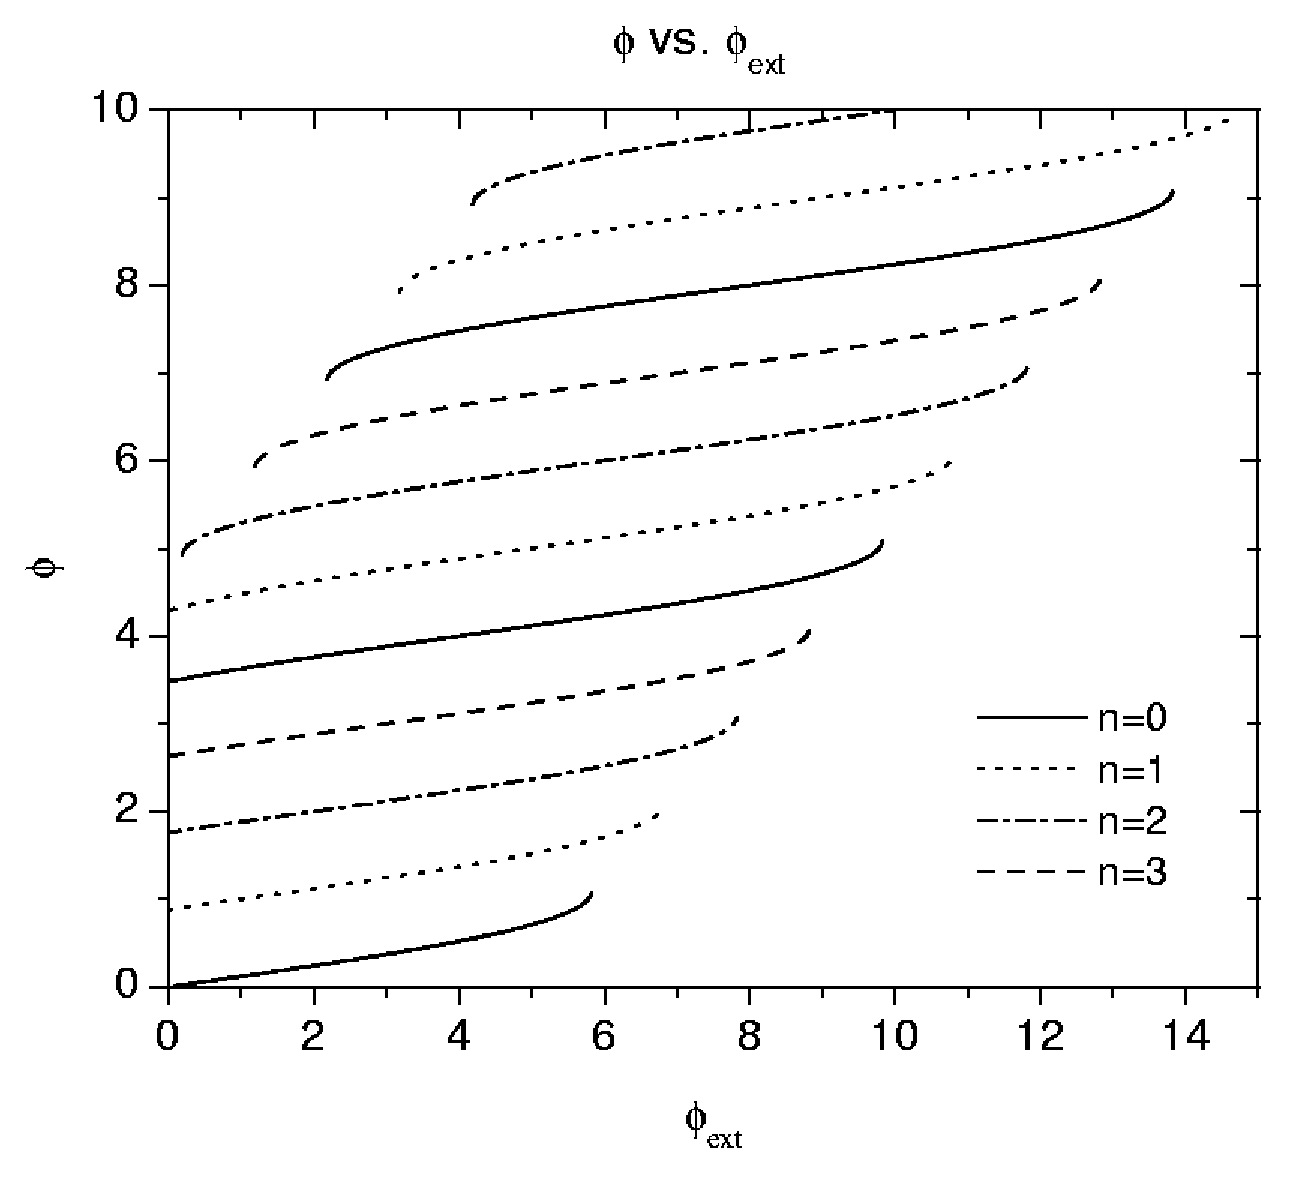
\includegraphics[width=5.7in]{figs/jjarray/chap2fig3.ps}
\caption[\phitot\ plotted against \phiext\ for $\betal= 30$
and $N=4$ for different values of the quantization number $n$.]
{\phitot\ plotted against \phiext\ from
\protect\EqnRef{eqn:steadystatesolution}\ for $\betal= 30$
and $N=4$ for different values of the quantization number $n$.
}
\label{fig:steady_state_multivariate_solution}
\end{figure}

\index{quantum number|)}

\subsection{Time independent external field}

To analyze 
\EqnRef{eqn:ode} we perform the standard stability analysis
\cite{ott} to find
that steady state solutions take the form of 
%
\begin{equation}
\label{eqn:steadystatesolution}
\phitot = \phiext + {\betal \over 2 \pi} \sin \left[{2 \pi \over N} (n -
                           \phitot) \right]
\mathrm{.}
\end{equation}
%
The right hand side can result in either single or multiple solutions,
depending upon the value of \betal. The crossover point depends 
upon $N$, and the solutions are single-valued for $\betal < N$ and
multi-valued for $\betal \geq N$. 
\FigRef{fig:steady_state_multivariate_solution}\ shows 
\EqnRef{eqn:steadystatesolution}\ plotted for large $\betal= 30$
which demonstrates that for a given \phiext\ there are many different
solutions for \phitot\ possible. The solutions for different values
of $n$ are sometimes referred to as the different ``branches'' of the
solution. For each of these branches, only the positively sloped 
parts are plotted, because these are the physically realizable solutions,
which will be discussed below. 

\subsubsection{$\pi$-junctions}
\index{\pijunction|(emph}
\label{sec:pijunction}

Another interesting possibility is the presence of an intrinsic 
phase shift in
the order parameter across the junction. This phase shift may occur
if \eg\ the junction is formed from misaligned grains of a superconductor
with \dwave\ symmetry. If the intrinsic phase shift across 
all the junctions sums to
$\pi$, \EqnRef{eqn:steadystatesolution}\ becomes modified to
%
\begin{equation}
\phitot = \phiext + {\betal \over 2 \pi} \sin \left[{2 \pi \over N} (n -
                           \phitot) - \pi \right]
\mathrm{.}
\label{eqn:steadystatepijunction}
\end{equation}
% 
This effect is commonly described as due to the presence of \pijunctions.
The important physical difference between \EqnRef{eqn:steadystatesolution}\
and \EqnRef{eqn:steadystatepijunction}\ is that at $\phiext = 0$,
\EqnRef{eqn:steadystatesolution}\ allows the loop to have zero magnetization
while \EqnRef{eqn:steadystatepijunction}\ forces the loop to be
magnetized. 
These two cases have been confirmed experimentally in two junction
SQUIDs
\cite{mathai_phdthesis,mathai_prl_74_4523_1995}. 

\index{\pijunction|)}

\label{jjarray:single_loop_mag}
Instead of plotting \phitot\ \vs\ \phiext\ as in 
\FigRef{fig:steady_state_multivariate_solution} it is useful
to also consider a plot of the normalized  
magnetization $\phimag = \phitot - \phiext$
\vs\ \phiext\ since it is the magnetization that is often measured
experimentally. This is shown in \FigRef{fig:single_loop_mag}. 
If we consider \EqnRef{eqn:steadystatesolution},
immediately one important fact springs forth: the larger \betal\ the
steeper the magnetization curves. This implies that small variations
in the external flux may create large variations in the total flux
of the single loop. Furthermore, it is clear from \FigRef{fig:single_loop_mag}\
that the single loop is equally likely to be either paramagnetic
or diamagnetic over the entire range of \phiext. 

%
% figure phimag vs. phiexternal
%
\begin{figure}[p]
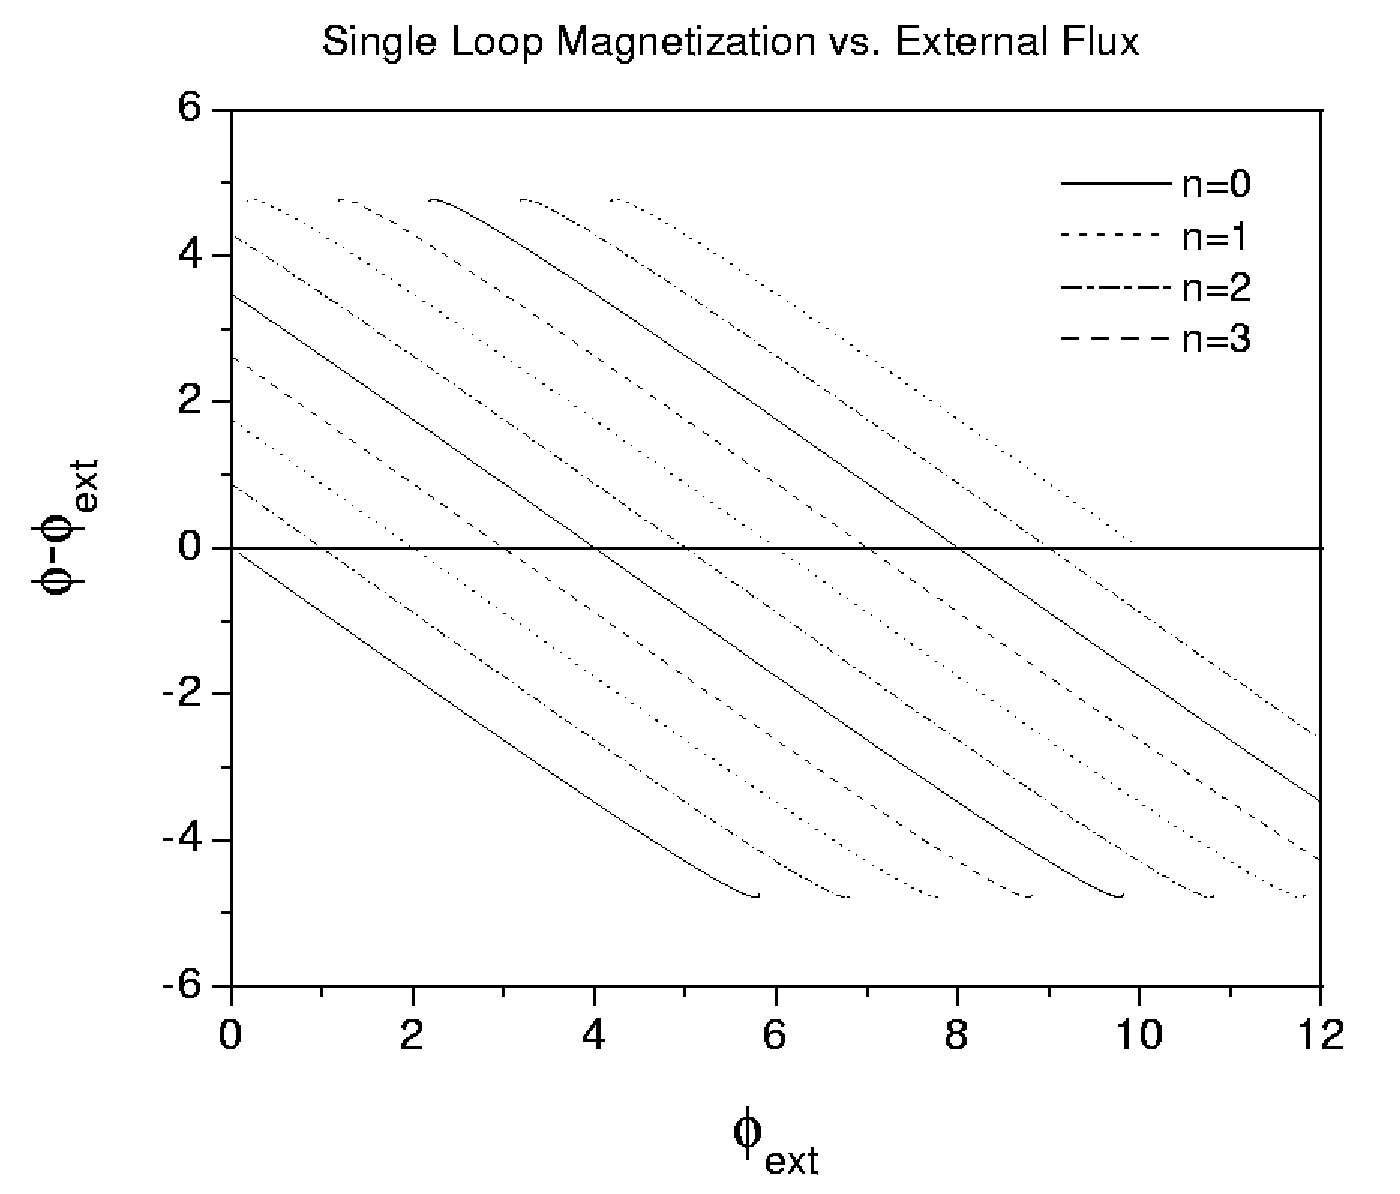
\includegraphics[width=5.7in]{figs/jjarray/phimag.ps}
\caption[Single loop magnetization \vs\ external flux.]
{Normalized magnetization
of a single loop, \phimag, plotted against the external flux \phiext\
applied to the loop for $\betal=30$ and $N=4$ for different values
of the quantization number $n$.}
\label{fig:single_loop_mag}
\end{figure}

Sigrist and Rice \cite{sigrist_jpsj_61_4283_1992,sigrist_rmp_503_67_1995}\
discussed the differences between
\EqnRef{eqn:steadystatesolution}\ 
and \EqnRef{eqn:steadystatepijunction}\ \visavis\ \swave\ and \dwave\ 
superconductivity for $N=1$ and concluded that observation of paramagnetism 
at $\phiext = 0$ provided evidence of a \pijunction\ in the
loop. However, they failed to account for the possibility that 
$\betal \gg N $ in \EqnRef{eqn:steadystatesolution}\ in which case
there are possible paramagnetic (and diamagnetic) 
solutions for \phitot\ at  $\phiext = 0$ even in the absence of 
\pijunction s. 

\EqnRef{eqn:steadystatesolution} does not tell the entire story.
For $\betal>N$ it specifies a multivalued solution with both
positive and negative slope. The solutions with positive slope are
seen experimentally, while those with negative slope are never seen.
This can be understood
by continuing the stability analysis of \EqnRef{eqn:ode}. 

%
% RSJ stability analysis
%
\label{RSJ model!stability analysis}
In the case of the RSJ model, \EqnRef{eqn:ode}\ reduces to 
%
\begin{equation}
\label{eqn:ode_rsj}
\phitot  = \phiext + {\betal \over 2 \pi} \left\{
         \sin\left[{2 \pi \over N}( n - \phitot)\right]
        - {2 \pi \over N} {\dif \phitot \over \dif \tau} 
        \right\}
\end{equation}
%
whose Jacobean has a single eigenvalue\footnote{For a complete discussion
of the stability analysis, see Ott \cite{ott}, p.~108.}
 of 
%
\begin{equation}
\label{eqn:rsj_eigenvalue}
\lambda =- {N\over 2 \pi} \left\{{2\pi\over\betal} + 
          {2\pi\over N} \cos \left[{2\pi\over N} (n-\phitot) \right] 
          \right\}
\end{equation}
%
For $\betal < N$, $\lambda$ will always be negative, hence any direction in 
\phitot\
from \EqnRef{eqn:ode}\ is a stable direction. This means that the loop
can settle into any value of \phitot\ for a given \phiext which 
solves \EqnRef{eqn:ode_rsj}. Additionally,
the solution to 
\EqnRef{eqn:ode_rsj}\
is single valued, so there is no ambiguity as to the state of the loop. 

In the case when $\betal > N$, $\lambda$ may change sign depending upon 
the particulars of the situation and $\lambda$ will be negative for 
%
\begin{equation}
\label{eqn:overdampedattracteigenvalue}
\cos\left[(n-\phitot) {2 \pi \over N} \right] > -{N \over \betal}.
\end{equation}
%
For $\lambda < 0$ the directions from the fixed point solutions
are stable directions so that the loop will stay in such a configuration. 
When $\lambda > 0$ the directions are unstable;  should any small thermal
fluctuation occur, a loop on the unstable 
fixed point solution will leave, and be
driven even further from the unstable solution. 


To illustrate this point, consider the first time derivative of 
\EqnRef{eqn:ode_rsj},
\begin{equation}
-\left\{1+{\betal\over N}\cos\left[(n-\phitot){2\pi\over N}\right]\right\}
{\dif\phitot\over\dif\tau} = {\betal\over 2\pi}{\dif^2\phitot\over\dif\tau^2}
\end{equation}
which takes the form of a moving particle experiencing a drag force. 
The ``drag coefficient''
\begin{displaymath}
-\left\{1+{\betal\over N}\cos\left[(n-\phitot){2\pi\over N}\right]\right\}
\end{displaymath}
takes a special form that is dependent upon \phitot, the position variable. 
Additionally,
the drag coefficient changes sign:  Instead of exerting drag, 
and slowing the particle, it pushes the particle and accelerates it 
away from \phitot. 
Conversely, when the drag 
coefficient is negative, the particle slows toward \phitot. The condition
for this switch over occurs at exactly the same place as the switch over
described for the eigenvalues above. 


%
% RCSJ stability analysis
%
\index{RCSJ model!stability analysis}
In the case of the RCSJ model, including $\betac$ in
\EqnRef{eqn:steadystatesolution}, makes the eigenvalues of the Jacobean 
more complicated,
but the same underlying behavior given by 
\EqnRef{eqn:overdampedattracteigenvalue}
occurs. The difference is that now while solutions are still
attracting or repelling, there are two types, depending on whether
or not the eigenvalues are complex or real. 
The eigenvalues themselves are given by
%
\begin{equation}
\label{eqn:fulleigenvalues}
\lambda_\pm = {N \over 4 \betac \pi} \pm {N \over 4 \betac} 
        \sqrt{1 + 8 \pi {\betac \over  \betal}
               + 2 \pi \betac \cos \left(\phitot {2 \pi \over N} 
                     \right)}
\end{equation}
%
The eigenvalues will
be purely real when
%
\begin{equation}
\label{eqn:undrivenrealeigen}
\cos \left[ (n-\phitot) {2 \pi \over N} \right] > - {1 \over 2 \pi \betac} 
                                              - {N \over \betal}
\mathrm{.}
\end{equation}
%
For sufficiently small \betal\ and \betac\ the eigenvalues will always 
be real and there will only be stable directions to the fixed point.
Additionally \EqnRef{eqn:undrivenrealeigen}\ 
reduces to the previous results for over damped junctions, if 
$\betac \rightarrow 0$. For large
enough \betal\ and \betac\ the fixed point solutions will have two
unstable directions. There is a range in between these
two possibilities in which the fixed point solutions have one stable
and one unstable direction. The unstable direction always dominates
in \EqnRef{eqn:fulleigenvalues}\ and the fixed point is  a
repulsor. 


\subsection{Time-dependent external field}

The single loop may also be put into a time-varying external field. 
The simplest case which may be considered, and the only case considered
here, is that of a sinusoidal 
driving field
%
\begin{equation}
\label{eqn:sindrive}
\phi_\mathrm{ac}(\tau) = \phiext \sin (\omega \tau)
\end{equation}
%
%We can separate \EqnRef{eqn:ode}\ into three first order autonomous 
%equations, when we substitutute \EqnRef{eqn:sindrive}\ for \phiext. 
%These are:
%\begin{eqnarray}
%{\dif \phiext' \over \dif \tau} & = & {8 \over \pi \betal \betac} \times \nonumber \\
% & & 
% \left[ -\phitot +\phiext\sin(f)+{\betal \over 2 \pi} \sin 
%     \left({n \pi \over 2} - {\pi \over 2}{\phitot \over \Phi_0} \right)
%   - {\betal \over 4} \phitot' \right] \\
%{\dif \phitot \over \dif \tau} & = & \phitot' \\
%{\dif f \over \dif \tau} & = & \omega .
%\end{eqnarray}

We can substitute \EqnRef{eqn:sindrive}\ for \phiext\ in to
\EqnRef{eqn:ode}\ and then analyze the result in different cases. 
It is useful to make the definition
\begin{equation}
\omega_0^{-2} = {\pi\over 8}\betal\betac , 
\end{equation}
where $\omega_0$
 corresponds to the dimensionless natural frequency of the system
if the non-linear \jj\ term is ignored. 
To see why this definition of $\omega_0$ is useful, consider 
rewriting \EqnRef{eqn:ode} in the form
%
\begin{equation}
\label{eqn:ode_reform}
{\pi\over 8}\betal\betac {\dif^2\phitot\over\dif\tau^2} = 
-\phitot + \phiext\sin(\omega\tau)-{\betal\over 4}{\dif\phitot\over\dif\tau}
+ {\betal\over 2\pi}\sin\left[ (n-\phitot){2\pi\over N} \right]
\end{equation}
%
which is clearly the form of a forced, damped harmonic
oscillator with an additional non-linear term. 


\subsubsection{Quasi-static case}

The quasi-static case is associated with $\phiext \ll {\betal/ 2 \pi}$ 
and 
$\omega \ll \omega_0$.
In this case the solutions are basically what we
expect for the static case. The system is driven so slowly and with such
low amplitude that it is always essentially in equilibrium. 
%There is no energy stored magnetically, all of the 
%energy is dissipated in the resistive channels in the junctions. 

%
% cut this section because I cannot justify it, nor do I think it's
% correct any longer. 
% 
%\subsubsection{Resonance}
%
%Resonance occurs when the driving frequency equals the natural
%frequency of the system $\omega_0 = \omega$. In this case, the non-linear
%term is irrelevant, and the loop operates essentially as a linear
%oscillator at resonance. 

\subsubsection{Large driving amplitude}

An interesting situation occurs when $\phiext \gg \betal / 2 \pi$. 
Here \phiext\ drives the loop so hard that the non-linear term is
irrelevant. This case corresponds to the loop responding simply as
a harmonic oscillator. 

\subsection{Gibbs free energy of single loop stable solutions}
\label{sec:gibbs_free_energy}

Assuming that the loop is able to achieve thermodynamic equilibrium
(which we have not generally assumed) the most favorable solution 
given by \EqnRef{eqn:steadystatesolution} would be the solution
\index{Gibbs free energy}
with the lowest Gibbs free energy. The Gibbs free energy in this case
is $\dif G = -I \dif\Phiext$\ \cite{silver_pr_157_317_1967,barone_and_paterno} 
which is easily determined 
numerically. 
This yields a series of Gibbs free energies for
each possible solution to \EqnRef{eqn:steadystatesolution}, with
the lowest Gibbs free energy corresponding to the solution which
has \phitot\ closest to \phiext. 
For the \phitot\ \vs\ \phiext\ curves in 
\FigRef{fig:steady_state_multivariate_solution} with $\betal = 30$, the
Gibbs free energy curves are plotted in
\FigRef{fig:gibbs_free_energy}.

\begin{figure}[p]
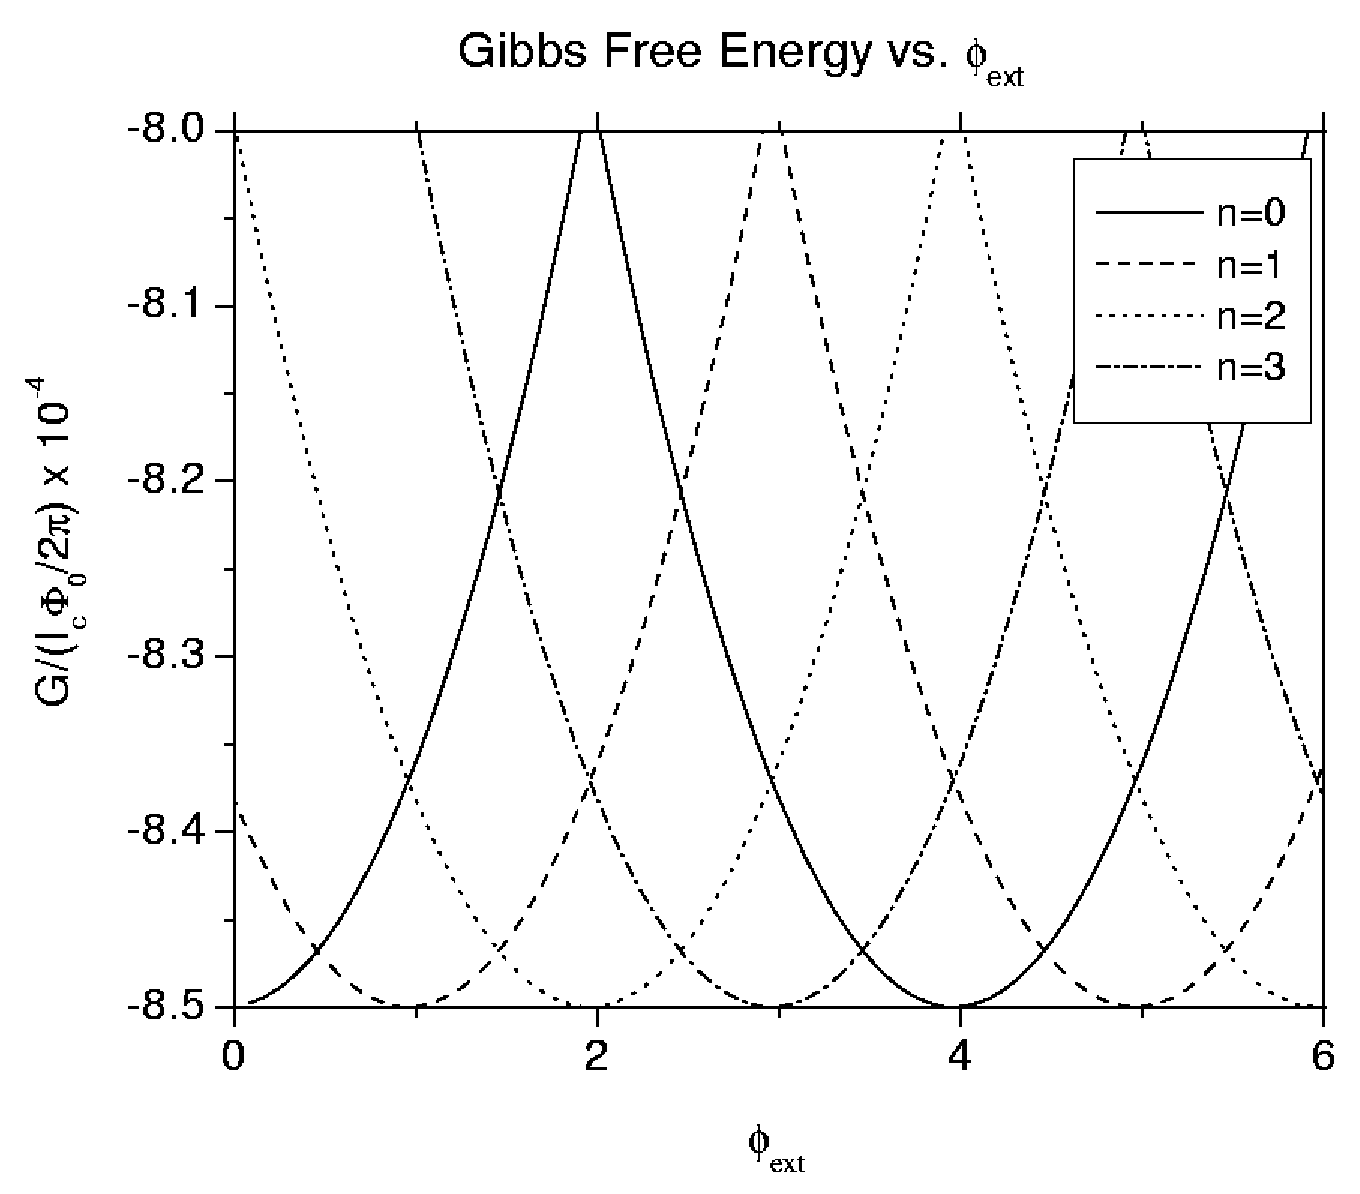
\includegraphics[width=5.7in]{figs/jjarray/chap2fig4.eps}
\caption{Gibbs free energy calculated for a four-junction loop with
$\betal = 30$.} 
\label{fig:gibbs_free_energy}
\end{figure}

\subsection{Non-identical junctions}
\label{sec:unsymmetric_junctions}

If we ignore the symmetry arguments which resulted in \EqnRef{eqn:ode}\
then for $N$ junctions in an isolated loop, for we will have $N$ equations to
solve. For each junction, \EqnRef{eqn:ftotvsfext} implies
%
\begin{equation}
{\phitot} = \phiext + {{\betal}_i\over 2 \pi} \sin \gamma_i
\label{eqn:ftotvsfext_indiv}
\end{equation}
%
in which ${\betal}_i$ is the $\betal$ parameter of the individual junction,
and accounts for individual junction variations in $I_c$ in the static 
case.  
In addition, the quantization rule, \EqnRef{eqn:fluxoidquant}, still holds.
We now substitute
\EqnRef{eqn:ftotvsfext_indiv} for 
\phitot\ to arrive at an equation for each junction, 
%
\begin{equation}
n-\phiext - {1\over 2\pi}\sum_i \gamma_i-{{\betal}_i\over 2\pi}\sin\gamma_i=0
\mathrm{.}
\end{equation}
%
The system must be solved numerically.
If one of the 
${\betal}_i$ is much larger than the others, then the loop behaves primarily
as a loop with $N-1$ junctions. For variance in ${\betal}_i$ on the order
of $10\%$, there is little change in the outcome, 
compared to the results for the
symmetric loop. 
This means that experiments on loops or \jjas\ with critical 
current
variations on the order of $10\%$ or less should exhibit behavior
similar to a uniform loop or array. Furthermore, models incorporating
uniform critical currents are significantly easier to implement.

This is significant because if small variations do not
affect the results very much, then
we expect that for a real \jja\ variations 
in the junction parameters on the order of $10\%$ will have only a small
bearing on the observations of those arrays. 

\section{Complete model of entire array}
\label{sec:entire_array_model}

% this figure shows the general outline for the array, including
% which junctions have which variables, etc. 
% this is a simple wire sketch, no islands etc. 
%
\begin{figure}[p]
\includegraphics{figs/jjarray/fig5.eps}
\caption[Sketch of \jja\ with labeled variables for numerical modeling.]
{Schematic arrangement for a square lattice \jja\ showing the 
variables used to describe each plaquette and junction in the
array. The positive direction for the loop currents are clockwise,
as indicated by the arrows, positive $\theta_{i,j}$ and $\gamma_{i,j}$
are measured in the vertical and horizontal direction respectively.}
\label{fig:array_model_sketch}
\end{figure}

To study the entire array, we take the same basic equations which describe
a single loop and scale them up.
In this section we will
consider a generic square lattice of $N \times M$ \jjsnoun, as depicted in 
\FigRef{fig:array_model_sketch}. \jjsnoun\ in the vertical
wires\footnote{The wires of the array are often refereed to as ``branches,''
while the loop currents are sometimes referred to as ``mesh'' currents.}
of the array are described by gauge-invariant phase difference 
$\theta_{j,k}$ and in the horizontal
wires by $\gamma_{j,k}$, while $I_{j,k}$ describes the loop current flowing
around each plaquette in the array. Considering loop currents simplifies
the analysis by eliminating the need to consider Kirchhoff's laws at each
intersection point of the array. 
For simplicity, consider here that the junctions are identical. 
With this arrangement, we may write an 
equation describing the current through each junction, using the normalizations
from the single loop case,
%
\begin{eqnarray}
\label{eqn:junc_horiz}
i_{j,k}-i_{j,k-1} & = & \sin\gamma_{j,k} +  {\dif\gamma_{j,k}\over\dif\tau}
                        + \betac {\dif^2\gamma_{j,k}\over\dif\tau^2} \\
i_{j,k}-i_{j-1,k} & = & \sin\theta_{j,k} + {\dif\theta_{j,k}\over\dif\tau} 
                        + \betac {\dif^2\theta_{j,k}\over\dif\tau^2} 
\label{eqn:junc_vert}
\end{eqnarray}
% 
as well as a quantization condition for each loop of the array,
%
\begin{equation}
\theta_{j,k} + \gamma_{j,k+1} - \gamma_{j,k} - \theta_{j+1,k} = 
 2 \pi n_{j,k} - 2 \pi \phi_{j,k} . 
\end{equation}
%
To fully define the array requires one further relation, the total flux
$\Phi_{i,j}$
threading the $i,j$ plaquette,
%
\begin{equation}
\phi_{j,k} = \phiext +{\betal\over 2 \pi} 
       \sum_{j',k'} m_{j,k,j',k'} \phi_{j',k'}
\label{eqn:total_flux_array}
\end{equation}
%
in which $m_{j,k,j',k'}$ is the mutual induction matrix between plaquette
$(j,k)$ and $(j',k')$ normalized to the self-inductance of a single plaquette,
$L$. 

The system detailed in Eqns.~(\ref{eqn:junc_horiz}) to 
(\ref{eqn:total_flux_array}) may also be condensed into a Hamiltonian
\index{Hamiltonian}
%
\begin{equation}
\mathcal{H} = \frac{1}{2}\betal 
           \sum_{j,k}\,m_{j,k,j',k'}\,{\phitot}_{j,k}\, i_{j,k}
    + \sum_{j,k} (1-\cos\gamma_{j,k})
    + \sum_{j,k} (1-\cos\theta_{j,k}),
\label{eqn:array_hamiltonian}
\end{equation}
%
where $\mathcal{H}$ is normalized to $\Phinot I_c / 2 \pi$. 
The sum in the first term is taken over each plaquette in the array while
the sums in the final two terms are taken over each junction in the array. 
This Hamiltonian will later be useful for investigating the energy 
landscape of the array. 

There have been many approaches to the solution of these equations
\cite{ebner_prb_31_165_1985,auletta_prb_47_14326_1993,%
auletta_prb_51_12844_1995,%
chandran_prb_56_6169_1997,%
filatrella_epjb_12_23_1999,lucheroni_prb_55_6559_1997} but perhaps
the most important result for the discussion here stems from work
by Phillips \etal \cite{phillips_prb_47_5219_1993}\ in which they 
show the importance of utilizing the full mutual induction matrix in order
to achieve accurate results. 

\subsection{Mutual induction matrix}
\index{induction matrix}

Because the full-induction matrix is just a geometrical property 
of the array it can in principle be computed. Phillips \etal\ put
forth one method to do this, on which this discussion will be based. 
There are two cases to consider when computing the matrix, the near
field, in which the physical extent of the plaquettes must be accounted 
for, and the far field, in which the plaquettes behave as current loops
composed of infinitesimal wires. 

\subsubsection{Near field}

We begin by modeling the array as a series of blocks (see 
\MultFigRef{fig:mutual_induction_matrix_blocks}{a}) and making 
the assumption
that the current density is uniform throughout the blocks.
Each block has
a uniform cross-sectional area $a$. The mutual induction matrix is then,
%
% the units of this are OK = Henry
\begin{equation}
\label{eqn:analytic_mutual_induction}
M_{j,k,j',k'} = {1\over a^2} {\mu_0\over 4 \pi} \oint\oint \dif\ell_{j,k}\,
  \dif\ell_{j',k'} 
  \int_A\int_{A'} {\dif a_{j,k}\, \dif a_{j',k'} \over \left|\vec r_{j,k} 
    - \vec r_{j',k'}\right|}
\end{equation}
%
which follows simply from Faraday's Law.\footnote{A very clear discussion
is given in Ramo, Whinnery and van~Duzer\cite{ramo_whinnery_vanduzer}, 
pp.~187-189.}
The integrals $\oint \dif\ell$ are taken around the two plaquettes 
of interest, the integrals $\int_A \dif a$ are taken over the facial area of
each block in the integration and $\mu_0$ is the magnetic constant.
\EqnRef{eqn:analytic_mutual_induction}\ 
cannot in general be integrated analytically, but can be integrated 
numerically
for the plaquettes of interest. 

%
% fig 2.6 -- geometry for mutual induction matrix
% 
\begin{figure}[p]
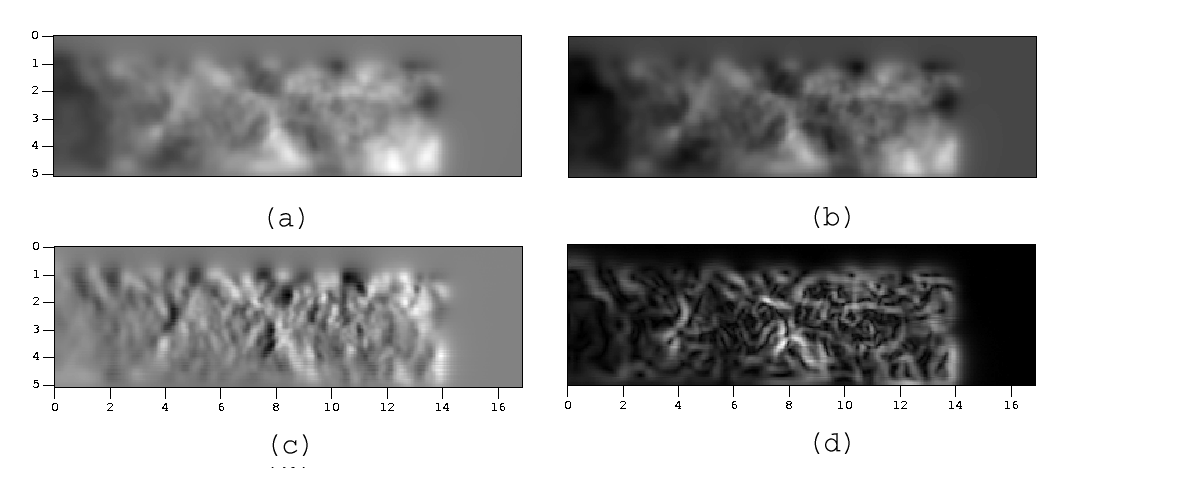
\includegraphics[width=5.7in]{figs/jjarray/fig6.ps}
\caption[Block arrangement used to compute mutual induction matrix.]
{Schematic of the block arrangement used to compute the
mutual induction matrix. (a) indicates the arrangement used for the 
near field, with $a_i$ representing the face of the block being
integrated over, $\ell_i$ representing the length around the loop 
integrated over, and $r$ representing the radius vector between the 
two blocks in the integration. (b) indicates the arrangement used 
to compute the mutual inductance in the far field. $r$ represents the
radius vector between the two loops and $\dif\ell_i$ represents the direction
of the integration around each loop.}
\label{fig:mutual_induction_matrix_blocks}
\end{figure}

\subsubsection{Far field}

In the far field \EqnRef{eqn:analytic_mutual_induction}\ simplifies
greatly to, as shown in \MultFigRef{fig:mutual_induction_matrix_blocks}{b},
%
% units of this equation are correct = Henry
\begin{equation}
M_{j,k,j',k'} = {\mu_0\over 4 \pi} {16 \sqrt{p} \over \sqrt{(j-j')^2 + (k-k')^2}}, 
\end{equation}
%
in which $p$ is the area of the plaquette,
which may be computed in a straight forward manner. 

It is complicated to compute the mutual induction matrix, but for a given
problem
we only need to compute the mutual induction matrix once.


% moved mean filed theory section to pme_theory.tex


